\section{\italics{Protein fold recognition}} \label{FRsection}

Al analizar secuencias gen\'{o}micas frecuentemente encontraremos marcos de lectura (te\'{o}ricos) que codifican para prote\'{i}nas que aparentemente no se parecen a ninguna otra (llamadas a veces \italics{orphans} en la literatura), 
o que s\'{o}lo tienen similitudes obvias con prote\'{i}nas de funci\'{o}n desconocida. Esto puede deberse a que de veras son 
mol\'{e}culas observadas por primera vez, o como vimos en \ref{3dcons}, a que la evoluci\'{o}n ha conservado en mayor grado
la estructura y topolog\'{i}a de las prote\'{i}nas hom\'{o}logas que sus secuencias. 

La segunda posibilidad ha justificado una familia de m\'{e}todos llamados gen\'{e}ricamente de \italics{Fold Recognition} (FR), 
que tienen como objeto reconocer a qu\'{e} tipo de plegamiento (de los conocidos) se debe asignar una secuencia problema, 
especialmente cuando b\'{u}squedas m\'{a}s convencionales con 
\htmladdnormallink{BLAST}{http://blast.ncbi.nlm.nih.gov/Blast.cgi} o 
\htmladdnormallink{FASTA}{http://www.ebi.ac.uk/Tools/fasta/index.html}
han fracasado.
Hist\'{o}ricamente algunos de estos m\'{e}todos se han llamado de
\htmladdnormallink{\italics{threading}}{http://en.wikipedia.org/wiki/Threading_\%28protein_sequence\%29}, 
ya que ciertos algoritmos 
literalmente enhebran la secuencia problema en patrones de coordenadas conocidas, normalmente un subconjunto no redundante
del PDB, para ver si es compatible con alguno, como en la siguiente figura:

\begin{figure}
\begin{center} 
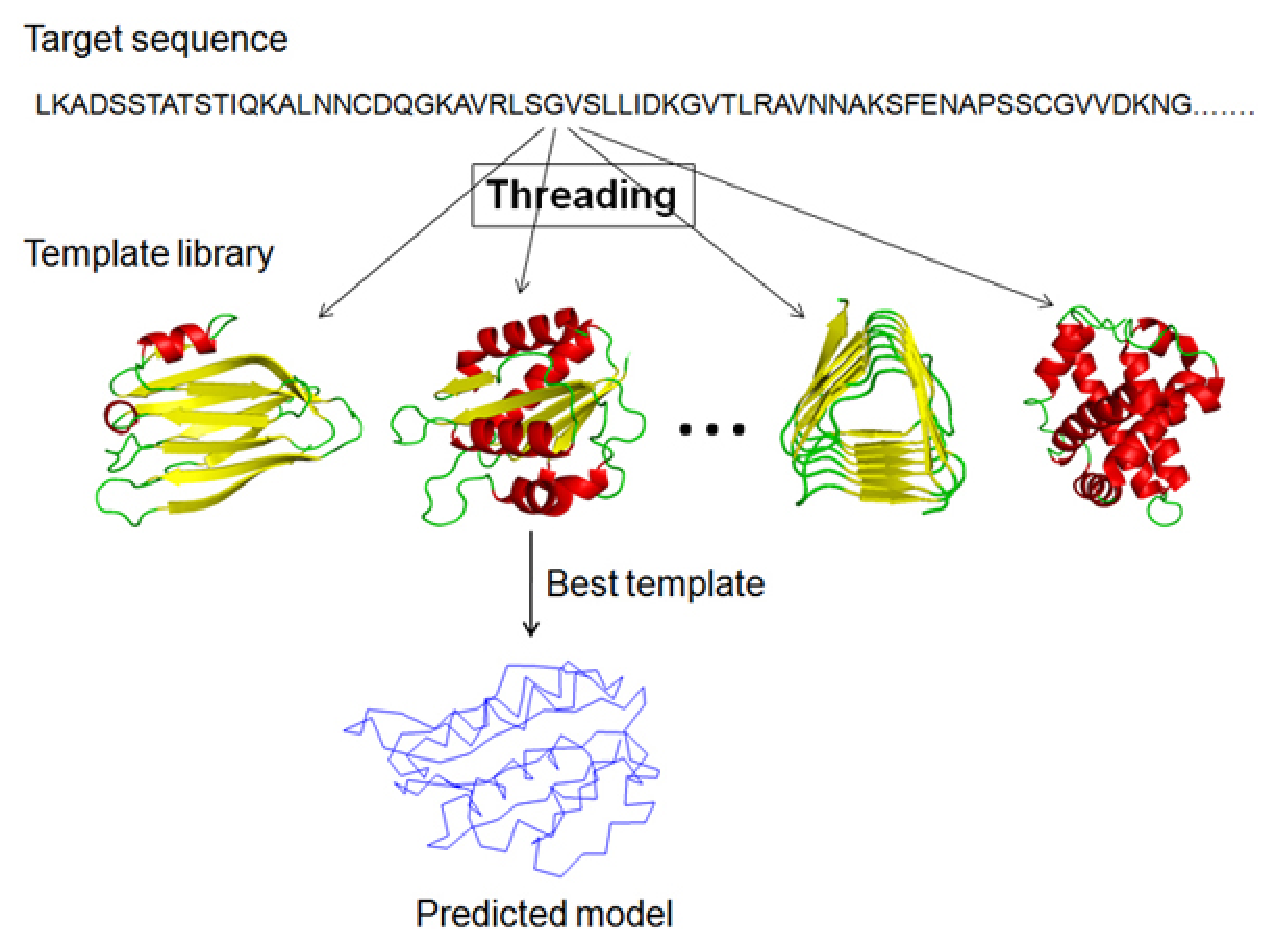
\includegraphics{threading}
\caption%[]
{
Diagrama de flujo de los algoritmos de reconocimiento de plegamiento (FR).
Figura tomada de \cite{Guo2008}. Copyright (2008) Frontiers in Bioscience. 
}
\label{fig:threading}
\end{center}
\end{figure}

El problema de FR lo podemos plantear as\'{i}:
\begin{itemize}
\item \textbf{PROBLEMA:} conocemos la secuencia de una prote\'{i}na, pero desconocemos su tipo de plegamiento y su funci\'{o}n
\item \textbf{SOLUCI\'{O}N PROPUESTA:} comparar la secuencia con todos los plegamientos conocidos, calcular el grado de parecido/compatibilidad con cada uno de ellos y devolver una lista ordenada
\end{itemize}

Se han publicado muchos algoritmos diferentes de FR; en todos ellos de alguna manera se asigna una estructura T a una secuencia A:
\begin{itemize}
\item Por medio de b\'{u}squedas PSI-BLAST bidireccionales transitivas \citep{Koretke2002}. 
La idea es que si buscamos secuencias hom\'{o}logas a partir de A llegamos a encontrar, en alguna iteraci\'{o}n, 
la secuencia T entre los resultados con cierta significancia estad\'{i}stica. De la misma manera, a partir de la secuencia de T llegamos a la secuencia A.

%(\htmladdnormallink{Pubmed}{http://www.ncbi.nlm.nih.gov/pubmed/12021456})
\item Representando cada plegamiento o \italics{fold} por medio de las secuencias conocidas que se pliegan en esa conformaci\'{o}n
y comparten estructura secundaria. Esto se puede hacer por medio de perfiles de secuencia \citep{Gribskov1987}, 
que son matrices sustituci\'{o}n de amino\'{a}cidos espec\'{i}ficas de posici\'{o}n, 
%\htmladdnormallink{perfiles}{http://www.ncbi.nlm.nih.gov/pubmed/3474607} 
o \htmladdnormallink{modelos ocultos de Markov}{http://en.wikipedia.org/wiki/Hidden_Markov_model}, 
que modelan expl\'{i}citamente con qu\'{e} probabilidad se pueden emitir secuencias compatibles con ese plegamiento.

\item Por medio de alineamientos secuencia-perfil %\htmladdnormallink{secuencia-perfil}{http://www.ncbi.nlm.nih.gov/pubmed/12169530} 
o los m\'{a}s sensibles perfil-perfil \citep{Soding2005} %\htmladdnormallink{perfil-perfil}{http://www.ncbi.nlm.nih.gov/pubmed/15531603}, 
que son la raz\'{o}n del \'{e}xito del servidor \htmladdnormallink{HHpred}{https://toolkit.tuebingen.mpg.de/#/tools/hhpred}.

\item Usando potenciales estad\'{i}sticos para evaluar la cercan\'{i}a de los residuos de una secuencia
dado un plegamiento (lo que llamamos \italics{threading} \citep{Threader1992}). Estos m\'{e}todos requieren precalcular,
sobre una colecci\'{o}n de plegamientos no redundantes, con qu\'{e} frecuencia y a qu\'{e} distancia se forman 
parejas de residuos en las estructuras conocidas. %(\htmladdnormallink{genTHREADER}{http://www.ncbi.nlm.nih.gov/pubmed/10191147})

%\item ombinando diferentes moldes, alineamientos y algoritmos en estrategias de b\'{u}squeda de consenso, 
%con la ayuda de m\'{e}tricas fiables como \htmladdnormallink{3D-Jury}{http://www.ncbi.nlm.nih.gov/pmc/articles/PMC2040163/} \citep{Ginalski2003}

%\item Partiendo la secuencia problema en fragmentos, como una estrategia divide y vencer\'{a}s, buscando la estructura
%mas probable para cada fragmento por \italics{threading} \citep{Wu2010}

\end{itemize}

Probablemente la mejor manera de evaluar objetivamente y elegir un m\'{e}todo de FR 
son experimentos colectivos a ciegas con secuencias cuyas estructuras experimentales se hacen p\'{u}blicas
tras las entrega de las predicciones. Hay dos tipos de experimentos de estipo: 
\htmladdnormallink{CASP}{http://predictioncenter.org/index.cgi?page=public_serv}, 
que mide bianualmente la competencia de los algoritmos de los grupos participantes, y 
\htmladdnormallink{CAMEO}{https://www.cameo3d.org}, que hace evaluaciones continuas no supervisadas.

En palabras de \citet{Kelley2015}, desarrollador principal de 
\htmladdnormallink{Phyre2}{http://www.sbg.bio.ic.ac.uk/phyre2}, uno de los m\'{a}s completos,
los mejores predictores tienen resultados indistinguibles en la mayor parte de los casos,
pero en los casos mas complejos desde hace tiempo destaca por su consistencia y 
superiores resultados \htmladdnormallink{I-TASSER}{http://zhanglab.ccmb.med.umich.edu/I-TASSER}.

%En la pr\'{a}ctica, a menudo los usuarios recurrimos a
%\htmladdnormallink{metaservidores}{http://en.wikipedia.org/wiki/Metaserver} como
%\htmladdnormallink{BioInfobank}{http://meta.bioinfo.pl}, desde donde podemos mandar una secuencia problema 
%a muchos servidores de FR, y lo que es m\'{a}s importante, donde podemos evaluar de una manera fiable 
%la calidad de los resultados usando m\'{e}tricas basadas en consensos, como 
%%\htmladdnormallink{2003}{http://bioinformatics.oxfordjournals.org/cgi/reprint/19/8/1015} y 
%\htmladdnormallink{3D-Jury}{http://www.ncbi.nlm.nih.gov/pmc/articles/PMC2040163/} \citep{Ginalski2003}, 
%como podemos comprobar inspeccionando la \htmladdnormallink{tabla de resultados}{http://meta.bioinfo.pl/queue.pl} de BioInfobank.

Estas herramientas web son adecuadas para estudiar unas pocas secuencias, pero si queremos hacer un experimento de FR 
a gran escala, entonces buena idea instalar localmente el software elegido, como por ejemplo
\htmladdnormallink{hh-suite}{https://github.com/soedinglab/hh-suite}, el software que da vida a 
\htmladdnormallink{HHpred}{https://toolkit.tuebingen.mpg.de/#/tools/hhpred}.

El siguiente programa es un prototipo de alineamiento perfil-perfil que usa adem\'{a}s predicciones de estructura secundaria (ver figura \ref{fig:psipred}) 
para guiar el alineamiento. Es un algoritmo de programaci\'{o}n din\'{a}mica, que puedes comprender mejor con ayuda 
del \htmladdnormallink{\italics{Sequence Alignment Teacher}}{http://protein.bio.puc.cl/websoftware/web/?sid=3} \citep{Ibarra2010}.

Para probarlo necesitaras descargar los archivos de entrada
(\htmladdnormallink{1ngk\_A.pssm}{./files/1ngk_A.pssm},
\htmladdnormallink{1s69\_A.pssm}{./files/1s69_A.pssm},
\htmladdnormallink{1ngk\_A.psipred}{./files/1ngk_A.psipred},
\htmladdnormallink{1s69\_A.psipred}{./files/1s69_A.psipred}):
\verbatiminput{code/prog3.2.pl}
